\documentclass[12pt,finnish]{exam}
\usepackage[utf8]{inputenc}
\usepackage{graphicx}
\usepackage[rightcaption]{sidecap}
\usepackage{wrapfig}
\usepackage{babel}
\usepackage{enumitem}
\usepackage{icomma}
\usepackage{amsmath}
\usepackage{amssymb}
\usepackage[T1]{fontenc}
\usepackage{tikz}
\setlist[enumerate,1]{leftmargin=*}

\begin{document}
 \section*{Integraalilaskenta (osio 1)}
\vspace{5mm}
 
\begin{questions}
\bfseries
\question
\mdseries
\begin{enumerate}[label=\textbf{\alph*)}]
\item Anna esimerkki jatkuvasta funktiosta \(f:[0, 1]\rightarrow \mathbb{R}\), jolla on ominaisuudet \(f(0)=f(1)=0\) ja \(\displaystyle \int_0^1 {f(x)} \text{ d}x=100\). \emph{(yo 2003k)}\\
\item Määritä käyrän \(y=-\ln x\) ja koordinaattiakselien rajoittaman alueen pinta-ala integroimalla \(y\):n suhteen.
\end{enumerate}

\bfseries
\question
\mdseries 

\vspace{-9ex}

\noindent\begin{minipage}{0.6\textwidth}

\vspace{11.2ex}
Nykytaiteen museorakennuksen pohja on ympyrä, jonka halkaisija on 19,7 metriä. Jos rakennus leikataan pohjaympyrän tietyn halkaisijan suuntaisella tasolla, leikkauskuvio on aina suorakulmio, jonka korkeus on puolet kannasta. Määritä rakennuksen tilavuus. \emph{(yo 2002s)}
\end{minipage}
\hfill%
\begin{minipage}{0.3\textwidth}% adapt widths of minipages to your needs

\vspace{10ex}
\includegraphics[width=\linewidth]{rakennus2}
\end{minipage}%



\bfseries
\question
\mdseries
Eräästä avaruuden pisteestä maapallo (säde \(R\)) havaitaan kulmassa \(\alpha\). Kuinka suuri alue maapallosta voidaan nähdä kyseisestä pisteestä? Määritä tämän kalotin pinta-ala integroimalla ja esitä se säteen \(R\) ja kulman \(\alpha\) funktiona.
\\  
\\ 
\\ 
\\
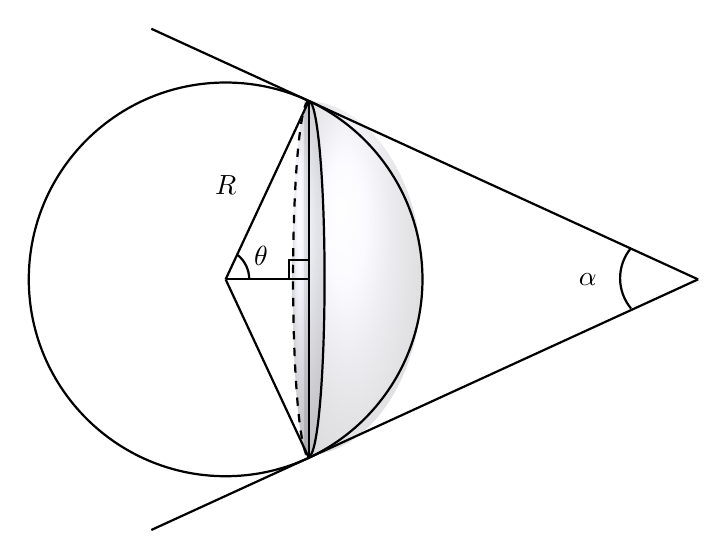
\begin{tikzpicture}
\shade[ball color=blue!10!white,opacity=0.2] (1,{2.5*sin(65)}) arc (90:-90:1.5cm and 2.25cm);
\shade[ball color=blue!10!white,opacity=0.2] (1.05,{2.5*sin(65)}) arc (90:270:0.2cm and 2.25cm);
\shade[ball color=blue!10!white,opacity=0.2] (1.05,{2.5*sin(65)}) arc (90:-270:0.2cm and 2.25cm);

\draw[black,thick] (0,0) circle (2.5 cm);
\draw[black,thick] (0,0) -- ({2.5*cos(65)},{2.5*sin(65)});
\draw[black,thick] (0,0) -- ({2.5*cos(65)},{-2.5*sin(65)});

\draw[black,thick] (6,0) -- ({2.5*cos(65)-2},{2.5*sin(65)-2*(2.5*sin(65))/(2.5*cos(65)-6)});


\draw[black,thick] (6,0) -- ({2.5*cos(65)-2},{-2.5*sin(65)+2*(2.5*sin(65))/(2.5*cos(65)-6)});

\draw[dashed,black,thick] ({2.5*cos(65)},{2.5*sin(65)}) arc (90:270:0.2cm and 2.2567cm);
\draw[black,thick] ({2.5*cos(65)},{2.5*sin(65)}) arc (90:-90:0.2cm and 2.2567cm);

\draw[black,thick] ({2.5*cos(65)},0) rectangle ({2.5*cos(65)-0.25},0.25);

\draw[black,thick] (0,0) -- ({2.5*cos(65)},0);
\draw[black,thick] ({2.5*cos(65)},{-2.5*sin(65)}) -- ({2.5*cos(65)},{2.5*sin(65)});

\draw[black,thick] (5.15,0.4) arc (140:220:0.6cm);

\draw[black,thick] (0.3,0) arc (0:50:0.4cm);

\node at (4.6,0) {\(\alpha\)};

\node at (0.45,0.3) {\(\theta\)};

\node at (0,1.2) {\(R\)};

\end{tikzpicture}


\end{questions}

\newpage

 \section*{Integraalilaskenta (osio 2)}
\vspace{5mm}
 
\begin{questions}
\bfseries
\question
\mdseries
Hissi lähtee liikkeelle levosta, ja sen liikettä kuvaa malli \(a(t)=2,0\cdot \sin{(0,4t)}\), jossa \(t\) on kulunut aika (s) ja \(a(t)\) on kiihtyvyys (m/s\(^2\)). 
\begin{enumerate}[label=\textbf{\alph*)}]
\item Määritä hissin suurin nopeus ja ajanhetki, jolla tämä saavutetaan ensi kerran.
\item Kuinka pitkän matkan hissi kulkee ensimmäisen 10 sekunnin aikana?
\item Määritä hissin keskinopeus edellisen kohdan aikavälillä.
\end{enumerate}

\bfseries
\question
\mdseries
Yksikkösäteinen, \((2, 2)\)-keskinen ympyrä pyörähtää täyden kierroksen \(x\)-akselin ympäri. 
\begin{enumerate}[label=\textbf{\alph*)}]
\item Laske kappaleen tilavuus integraalilaskennan avulla.
\item Osoita väite oikeaksi tai vääräksi: tilavuus on pyörähdyspinnan alan ja sen\\ painopisteen kulkeman matkan tulo.
\end{enumerate}

\bfseries
\question
\mdseries
Kuinka suuren työn voima \(\displaystyle F=ma=m\frac{\mathrm{d}v}{\mathrm{d}t}\) tekee siirtäessään kappaletta matkan \(\mathrm{d}s\)? Laske, kuinka paljon työtä tehdään, kun kappale kiihdytetään nopeudesta \(v_1\) nopeuteen \(v_2\). Mitä huomaat?

\end{questions}
\thispagestyle{empty}

\end{document}

